% KEYSTONE: supplementary material for the JCS submission (anonymized).
% Full proofs of the results stated with proof sketches in the article, and the
% figures and tables moved out of the article for length. Numbers of theorems,
% lemmas and equations refer to the article.
\documentclass[11pt]{article}
\usepackage[a4paper,margin=2.5cm]{geometry}
\usepackage{amsmath,amssymb,amsthm}
\usepackage{booktabs,array,tabularx,graphicx}
\usepackage[numbers,sort&compress]{natbib}
\usepackage{url}
\usepackage[hidelinks]{hyperref}
\graphicspath{{../figures/}{../../r1/figures/}}

\newtheorem*{lemmaS}{Lemma}
\newtheorem*{theoremS}{Theorem}
\newtheorem*{propositionS}{Proposition}
\renewcommand{\thefigure}{S\arabic{figure}}
\renewcommand{\thetable}{S\arabic{table}}

\newcommand{\G}{\mathbb{G}}
\newcommand{\Zq}{\mathbb{Z}_\ell}
\newcommand{\PAC}{\mathrm{PAC}}

\title{KEYSTONE: Readiness Audits for Dispute-Key Availability in Encrypted Rollups\\[4pt]
\large Supplementary material}
\author{[Author details removed for peer review]}
\date{}

\begin{document}
\maketitle

\noindent This supplement gives full proofs of the results that the article states with proof sketches (Lemmas~1--4, Corollary~2, Theorems~2 and~3 with the limit after accepted audits, and Propositions~3 and~4), the stratified-sampling formula (Proposition~S1), and figures and tables moved out of the article for length. Notation follows the article; assumption, lemma, theorem and equation numbers refer to it. The temporal results are exact under the declared model; their parameters are synthetic.

\section{Proofs for the audit (Lemmas 1--3)}

\begin{lemmaS}[Lemma 1, correctness and knowledge soundness]
An honest response passes verification. In the random-oracle model a verifying response satisfies $D_i=X^{x_i}$ except with negligible probability, and the proof is a proof of knowledge. Any $t$ verified partials of $C_1$ with distinct indices $I$ combine to $PK_E^{\rho}$.
\end{lemmaS}

\begin{proof}
Completeness: $g^{z}=g^{\nu+cx_i}=a_1Y_i^{c}$ and $X^{z}=a_2D_i^{c}$ when $D_i=X^{x_i}$. The Chaum--Pedersen protocol is special-sound: two accepting transcripts with one commitment and different challenges $c\neq c'$ give $x_i=(z-z')/(c-c')$, and the same pair shows $D_i=X^{x_i}$. With the Fiat--Shamir hash as a random oracle, the forking lemma turns a party that produces verifying proofs for fresh canaries with non-negligible probability into an extractor that obtains $x_i$, and value soundness follows\cite{chaum1992dleq,fiat1987prove}. Combination: $\prod_{i\in I}C_1^{x_i\lambda_i^I}=C_1^{x}=g^{\rho x}=PK_E^{\rho}$.
\end{proof}

\begin{lemmaS}[Lemma 2, simulatable audit transcripts]
Model $H_G$ and $H$ as random oracles. A simulator that knows only $g$ and $Y_1,\dots,Y_n$ answers all oracle queries and produces honest custodians' audit responses for any audit context and sample. With at most $N$ simulated proofs and $Q$ oracle queries, simulated and real views are within statistical distance $NQ/\ell$, so observing audits changes any adversary's advantage against $\PAC$ by at most $2NQ/\ell$.
\end{lemmaS}

\begin{proof}
The simulator answers every fresh $H_G$ query, from the protocol or the adversary, with $g^{a}$ for a stored $a\leftarrow\mathbb{Z}_\ell^{*}$, which is exactly a random oracle onto $\G\setminus\{1\}$. For an honest custodian and canary $X=g^{a}$ it sets $D_i=Y_i^{a}=X^{x_i}$, the real response. Each proof comes from the honest-verifier zero-knowledge simulator: draw $c,z\leftarrow\Zq$, set $a_1=g^{z}Y_i^{-c}$ and $a_2=X^{z}D_i^{-c}$, and program $H$ at that input to $c$. Since $a_1$ is uniform, the input was queried before with probability at most $Q/\ell$, and a union bound over $N$ proofs gives the distance. Corrupted custodians' responses come from the adversary. Because $H$, $H_G$ and the key-derivation function are independent and domain separated, this programming does not interfere with a reduction to the KEM that programs the key-derivation oracle, so an adversary against $\PAC$ that sees audits becomes one against the KEM alone, the probability of each output moving by at most $NQ/\ell$.
\end{proof}

\begin{lemmaS}[Lemma 3, no production substitution]
For a fixed $C_1$, a coordinator making $Q$ queries to $H_G$ finds an audit context whose canary equals $C_1$ with probability at most $Q/(\ell-1)$.
\end{lemmaS}

\begin{proof}
Each query returns an independent uniform element of $\G\setminus\{1\}$, equal to the fixed $C_1\neq1$ with probability $1/(\ell-1)$; apply the union bound.
\end{proof}

\begin{propositionS}[S1, stratified samples]
Partition the committee into failure domains $G_1,\dots,G_h$ of sizes $n_j$ with $k_j$ audit-ready custodians, and sample $s_j$ custodians uniformly without replacement from each $G_j$, independently, with $\sum_j s_j=s$. Then
\[
\Pr[\mathsf{accept}]=\sum_{\substack{(i_1,\dots,i_h)\\ i_1+\dots+i_h\ge q}}\ \prod_{j=1}^{h}\frac{\binom{k_j}{i_j}\binom{n_j-k_j}{s_j-i_j}}{\binom{n_j}{s_j}}.
\]
\end{propositionS}

\begin{proof}
The per-domain counts of ready sampled custodians are independent hypergeometric $(n_j,k_j,s_j)$ variables, and the audit accepts if and only if their sum is at least $q$.
\end{proof}

\section{Proof of Lemma 4 (record-bound releases)}

\begin{lemmaS}[Lemma 4]
Let the dispute KEM be TDH2 with label $L_r=(E,\mathsf{id}_r,\text{policy hash})$, and let each custodian release $C_1^{x_i}$, with its DLEQ proof, only for a ciphertext whose TDH2 proof verifies and whose label is the authorized one. Under Assumptions~1 and~5 and static corruption of fewer than $t$ custodians, $\PAC^{+}$ holds for every record, and Lemma~2 continues to hold.
\end{lemmaS}

\begin{proof}
Record identifiers are unique (Assumption~3), so distinct records have distinct labels. Fix a target record $r$ and an adversary $\mathcal{A}$ against $\PAC^{+}$. In \emph{Game~0}, the $\PAC^{+}$ experiment, $\mathcal{A}$ chooses two equal-length plaintexts $m_0,m_1$ for $r$; the challenger seals $m_b$ for a uniform bit $b$; $\mathcal{A}$ sees the public key, the public shares, the corrupted custodians' shares, all audit transcripts, the sealed target and the releases of every other record, including records it commits itself, and outputs a guess $b'$. Let $\mathrm{Adv}=|\Pr[b'=b]-\tfrac12|$.

\emph{Game~1} replaces the honest custodians' audit responses by the simulator of Lemma~2; by Lemma~2 and domain separation, $\Pr[b'=b]$ moves by at most $NQ/\ell$.

\emph{Game~2} replaces the target's key-encryption key $\kappa_r=\mathrm{KDF}(PK_E^{\rho},L_r)$ by a uniform key. The dispute ciphertext is a tag-KEM/DEM hybrid\cite{abe2008tagkem}: TDH2's threshold key encapsulation, whose proof hashes the label and the wrapped key as its tag, with $\kappa$ as encapsulated key and AES-GCM as data encapsulation. A reduction $\mathcal{B}$ to Assumption~5, the chosen-ciphertext security of this tag-KEM, bounds the change. In the threshold model of Shoup and Gennaro\cite{shoup2002securing}, who prove the corresponding property of TDH2 encryption under DDH in the random-oracle model, $\mathcal{B}$ receives the public key, the public shares and the corrupted shares, and forwards them. It obtains the challenge encapsulation for label $L_r$ with a key $\kappa^{*}$ that is either the real one or uniform, wraps a fresh data key $K_r$ under $\kappa^{*}$ with AES-GCM and associated data $L_r$, encrypts $m_b$ under $K_r$, and gives $\mathcal{A}$ the sealed target. Audits are simulated as in Game~1, without the secret key. A release request for a record $r'\neq r$ concerns a ciphertext with label $L_{r'}\neq L_r$. If its TDH2 proof does not verify, honest custodians refuse it, as in the protocol. Otherwise it differs from the challenge at least in its label, so $\mathcal{B}$ obtains all decryption shares, with their proofs, from its oracle and computes the combined value by Lagrange interpolation, which is everything a release delivers. No release with label $L_r$ is answered, because $r$ is not released in the $\PAC^{+}$ game, and the target's components under another label form a different ciphertext, valid only if its proof, which hashes the label, verifies; the chosen-ciphertext game permits such a query, and Assumption~5 is exactly the statement that no efficient adversary gains from it. $\mathcal{B}$ outputs $1$ if $b'=b$, so the change is at most the advantage against Assumption~5.

\emph{Game~3} wraps a fixed all-zero key instead of $K_r$. Because $\kappa^{*}$ is uniform and used once, the change is at most the advantage against AES-GCM as a one-time secure data encapsulation, the step the tag-KEM/DEM composition theorem\cite{abe2008tagkem} makes generic. Now $K_r$ is used only to encrypt $m_b$.

\emph{Game~4} encrypts $m_0$ instead of $m_b$ under the uniform, once-used $K_r$; the change is at most the AES-GCM advantage, and in Game~4 the view is independent of $b$. Summing,
\[
\mathrm{Adv}\le \frac{NQ}{\ell}+\mathrm{Adv}^{\mathrm{cca}}_{\mathrm{TDH2\text{-}tagKEM}}+2\,\mathrm{Adv}^{\mathrm{ae}}_{\mathrm{AES\text{-}GCM}},
\]
which is negligible under Assumptions~1 and~5. The canary path does not use the KEM and its oracles are domain separated from the TDH2 oracles, so Lemma~2 holds unchanged. Proposition~1 shows that the label and validity checks are necessary: without them, the release of a re-submitted $C_1$ under a fresh identifier answers the challenge.
\end{proof}

\section{Proof of Corollary 2 (stochastic deadline)}

\begin{lemmaS}[Corollary 2]
Suppose $n_\ell$ custodians can answer, each response is delivered independently with probability $p_\ell$ after a round trip with distribution function $F$, and the combiner finishes within $B$ after the $t$-th valid response. Then $\Pr[\mathrm{DDL}(r,E,\tau,\Delta_d)]\ge\Pr[\mathrm{Bin}(n_\ell,p_\ell F(\Delta_d-B))\ge t]$.
\end{lemmaS}

\begin{proof}
Each of the $n_\ell$ responses is delivered within $\Delta_d-B$ of the request independently with probability $p_\ell F(\Delta_d-B)$, so their number $M$ is $\mathrm{Bin}(n_\ell,p_\ell F(\Delta_d-B))$. On the event $M\ge t$, the $t$-th valid response arrives by $\tau+\Delta_d-B$ and the combiner finishes by $\tau+\Delta_d$, so $\mathrm{DDL}$ holds.
\end{proof}

\noindent In the R2b replication, $F$ is the law of the injected two-leg delay, $p_\ell=(1-\mathrm{loss})^2$, and $B$ is the 99th percentile of the dispute completion time at zero injected delay, which absorbs transport, decoding and the combiner's work. $B$ is therefore a high quantile rather than a bound, and the 0.99 target of $\Delta_{os}$ is approximate; the replication tests it on fresh traces.

\section{Proofs for readiness over time}

\paragraph{Model.} Each of $n$ custodians is an independent two-state continuous-time Markov chain with failure rate $\phi>0$ and repair rate $\psi>0$; $v=\psi/(\phi+\psi)$, and $p_{\uparrow}(u)=v+(1-v)e^{-(\phi+\psi)u}$ and $p_{\downarrow}(u)=v(1-e^{-(\phi+\psi)u})$ are the probabilities of being up at $u$ given up, respectively down, at $0$; note $p_{\uparrow}(u)-p_{\downarrow}(u)=e^{-(\phi+\psi)u}\ge0$. In the domain-shock variant, $h$ domains of $n_0=n/h$ custodians each follow a further independent two-state chain with rates $\phi_d,\psi_d>0$, and a custodian is ready when it and its domain are up. Faults are non-selective, audits at $T,2T,\dots$ draw fresh uniform samples and trigger no repair, and disputes arrive independently of the process. $A(k)$ is the acceptance probability of Eq.~(1) of the article, non-decreasing in $k$.

\begin{lemmaS}[Lumped chains]
(i) Without domain shocks, the number $Z$ of ready custodians is a Markov chain with kernel
\[
P_u(k,k')=\sum_i\mathrm{b}(i;k,p_{\uparrow}(u))\,\mathrm{b}(k'-i;n-k,p_{\downarrow}(u))
\]
and stationary law $\omega=\mathrm{Bin}(n,v)$. (ii) With domain shocks, the process $X=((\delta_j,J_j))_{j=1}^{h}$, where $\delta_j$ indicates that domain $j$ is up and $J_j$ counts its members that are individually up, is a Markov chain whose kernel is the product of the per-domain kernels $P^{\delta}_u\otimes P^{(n_0)}_u$, and $Z=\sum_j\delta_jJ_j$.
\end{lemmaS}

\begin{proof}
(i) The configuration process is a product of independent two-state chains. Started from a configuration with $k$ custodians up, after time $u$ each of them is up independently with probability $p_{\uparrow}(u)$ and each of the $n-k$ others with probability $p_{\downarrow}(u)$, so $Z(u)$ is the sum of independent $\mathrm{Bin}(k,p_{\uparrow}(u))$ and $\mathrm{Bin}(n-k,p_{\downarrow}(u))$ variables. This law depends on the configuration only through $k$, which is Dynkin's criterion for strong lumpability; hence $Z$ is Markov with kernel $P_u$. Each custodian's stationary law is $(1-v,v)$, and independence gives $\omega=\mathrm{Bin}(n,v)$. (ii) Domains are mutually independent, and inside a domain the domain chain is independent of the member chains; applying (i) inside each domain lumps its members to $J_j$, and lumping commutes with the product because the blocks are independent. A custodian is ready if and only if it and its domain are up, so $Z=\sum_j\delta_jJ_j$.
\end{proof}

\noindent The pair (domain states, $Z$) is a function of $X$ but not Markov in general: two configurations with the same domain states and the same $Z$ whose down domain has different $J_j$ have different futures once that domain recovers. Below, ``the chain'' is $Z$ without shocks and $X$ with shocks, $\omega$ its stationary law, and $A$, $\mathbf{1}_{<t}$ are read as functions of its state through $Z$.

\begin{theoremS}[Theorem 2, risk given an audit history]
Let the process be stationary before the first audit, and for outcomes $o_1,\dots,o_j$ let $\alpha_1\propto\omega\odot e_{o_1}$ and $\alpha_i\propto(\alpha_{i-1}P_T)\odot e_{o_i}$, normalized, with $e_{\mathsf{acc}}=A$ and $e_{\mathsf{rej}}=1-A$. Then $\alpha_j(x)=\Pr[X(jT)=x\mid o_1,\dots,o_j]$, and for $0\le u<T$, $\Pr[Z(jT+u)<t\mid o_1,\dots,o_j]=\alpha_jP_u\mathbf{1}_{<t}$.
\end{theoremS}

\begin{proof}
By the lemma, the chain sampled at the audit times is a Markov chain with kernel $P_T$. Given the path, the $i$-th sample is fresh, uniform and independent of everything else, and faults are non-selective, so $o_i$ is conditionally independent of all other variables given the state at $iT$ and is an acceptance with probability $A(Z(iT))$: the number of ready custodians in a uniform sample is hypergeometric and depends on the configuration only through $Z$. The audit history is therefore a hidden Markov model, and the recursion is Bayes' rule applied one audit at a time (the forward algorithm). For the dispute, the Markov property at $jT$ and the independence of the dispute time give the law $\alpha_jP_u$ at $jT+u$; summing over states with $Z<t$ gives the claim.
\end{proof}

\begin{propositionS}[Limit after accepted audits]
If all audits accept, $\alpha_j$ converges geometrically, from any start, to the normalized left Perron vector $\alpha^{*}$ of $M=P_T\,\mathrm{diag}(A)$ restricted to the states $S$ with $A>0$.
\end{propositionS}

\begin{proof}
For $T>0$, $0<p_{\downarrow}(T)<v<p_{\uparrow}(T)<1$, so each row of $P_T$ is the convolution of two binomial laws with full supports $\{0,\dots,k\}$ and $\{0,\dots,n-k\}$, which has full support $\{0,\dots,n\}$; hence $P_T>0$ entrywise. In the domain variant, each per-domain kernel is a Kronecker product of positive matrices and is positive, and so is their product. After one accepted audit, $\alpha$ is supported in $S$, and $M$ restricted to $S\times S$ is strictly positive. By the Perron--Frobenius theorem, $M$ has a simple dominant eigenvalue with a positive left eigenvector, and normalized iterates from any nonnegative nonzero start converge to it geometrically, by Birkhoff's contraction of the Hilbert projective metric.
\end{proof}

\begin{theoremS}[Theorem 3, undetected failure]
Let $U(T)=\frac1T\int_0^T(\omega\odot A)P_u\mathbf{1}_{<t}\,du$. With or without domain shocks, $U$ is non-decreasing in $T>0$ and $U(T)\ge U_0=(\omega\odot A)\mathbf{1}_{<t}$, which is its limit as $T\to0$. Without domain shocks,
\[
U(T)\le A(t-1)\,\omega(Z<t)+\sum_{k\ge t}\omega(k)A(k)\Pr[\mathrm{Bin}(k,p_{\uparrow}(T))<t],
\]
and the right-hand side is non-decreasing in $T$.
\end{theoremS}

\begin{proof}
\emph{Interpretation.} By stationarity, the independence of the dispute time and Theorem~2 with one audit, $U(T)$ is the long-run probability that a dispute fails and the most recent audit accepted.

\emph{Monotonicity and floor.} Order the states coordinatewise ($Z$ without shocks; each $\delta_j$ and $J_j$ with shocks), so that $A$ is non-decreasing and $h_0=\mathbf{1}_{<t}$ is non-increasing; with shocks this holds because $Z=\sum_j\delta_jJ_j$ is non-decreasing in every coordinate. The chain has three properties.
(a) It is reversible with respect to $\omega$: each coordinate is a two-state chain or a birth--death chain, both reversible, and a product of independent reversible chains is reversible.
(b) Every transition changes one coordinate by one step.
(c) $P_u$ maps non-increasing functions to non-increasing functions: for a two-state chain this is $p_{\uparrow}(u)\ge p_{\downarrow}(u)$; for a birth--death count, raising the start by one replaces a $\mathrm{Bin}(1,p_{\downarrow})$ summand by a $\mathrm{Bin}(1,p_{\uparrow})$ one, a stochastically larger variable; and a product of independent monotone kernels is monotone.
Let $\mathcal{L}$ be the generator, $\langle f,h\rangle_{\omega}=\sum_x\omega(x)f(x)h(x)$, and $g(u)=(\omega\odot A)P_uh_0=\langle A,P_uh_0\rangle_{\omega}$. Then $g'(u)=\langle A,\mathcal{L}P_uh_0\rangle_{\omega}=-\mathcal{E}(A,P_uh_0)$, where by (a)
\[
\mathcal{E}(f,h)=\tfrac12\sum_{x,y}\omega(x)\,\mathcal{L}(x,y)\,\big(f(y)-f(x)\big)\big(h(y)-h(x)\big)
\]
is the Dirichlet form. By (b), each pair $x,y$ with $\mathcal{L}(x,y)>0$ is comparable; by (c), $P_uh_0$ is non-increasing; so each term has $(A(y)-A(x))((P_uh_0)(y)-(P_uh_0)(x))\le0$, and $g'(u)\ge0$. Hence $g$ is non-decreasing, its running mean $U(T)$ is non-decreasing in $T$, and $U(T)\ge g(0)=(\omega\odot A)h_0=U_0$. As $T\to0$, $P_u\to I$ and $g$ is continuous, so $U(T)\to U_0$.

\emph{Bound.} Without shocks, split $U$ by the state $k=Z(0)$ at the audit. For $k<t$, bound $\Pr_k[Z(u)<t]\le1$ and use $A(k)\le A(t-1)$. For $k\ge t$, let $N(u)$ count the $k$ custodians up at $0$ that are up at $u$. Then $Z(u)\ge N(u)$, since custodians down at $0$ can only add, and $N(u)\sim\mathrm{Bin}(k,p_{\uparrow}(u))$, so $\Pr_k[Z(u)<t]\le\Pr[\mathrm{Bin}(k,p_{\uparrow}(u))<t]$. Since $dp_{\uparrow}/du=-(1-v)(\phi+\psi)e^{-(\phi+\psi)u}<0$ and the binomial law is stochastically increasing in its success probability, this is at most $\Pr[\mathrm{Bin}(k,p_{\uparrow}(T))<t]$ for $u\le T$; averaging over $u$ keeps the bound, and the same two facts make the right-hand side non-decreasing in $T$.
\end{proof}

\noindent Consequently, a target $\varepsilon<U_0$ is unattainable at every interval, and $T^{*}(\varepsilon)=\sup\{T:U(T)\le\varepsilon\}$ is well defined and found by bisection; the runner bisected $\log T$ over $[0.25\,\mathrm{h},30\,\mathrm{d}]$. The interval from the bound is conservative. Monotonicity of the posterior risk $R(T)$ is not proved; its intervals rest on a numerical check of 25 points per cell, which passed in every cell.

\section{Proofs for repair on alarm and selective withholding}

\begin{propositionS}[Proposition 3, repair on alarm]
Let a rejected audit at time $a$ trigger a resharing that makes every custodian individually ready at $a+D_r$, with $0\le D_r\le T$, leaving domain states unchanged. Then the state just before audits is a Markov chain with kernel $M=\mathrm{diag}(A)P_T+\mathrm{diag}(1-A)P_{D_r}\Pi P_{T-D_r}$, where $\Pi$ is the reset map, and with $\mu$ its stationary law the long-run probability that a dispute fails is $F_{\mathrm{rep}}(T)$ as stated in the article, and resharings occur at rate $\mu_r\mathbf{1}/T$.
\end{propositionS}

\begin{proof}
Condition on the state $x$ just before an audit at $a$. The audit accepts with probability $A(x)$, independently of everything else given $x$ (Theorem~2). If it accepts, no action follows and the state at $a+T$ has law $\delta_xP_T$. If it rejects, the state evolves for $D_r$, the reset $\Pi$ is applied, and it evolves for $T-D_r$, giving law $\delta_xP_{D_r}\Pi P_{T-D_r}$. Because $D_r\le T$, every repair completes before the next audit, so the next pre-audit state depends only on $x$ and the outcome; summing over outcomes gives the kernel $M$. The kernel is primitive: for $T>D_r$ every row of $P_T$ and of $P_{T-D_r}$ is positive on the chain's support (Theorem~2), and for $T=D_r$ every row reaches the reset state, from which $P_T$ is positive. Hence $\mu$ exists, is unique and is the limit from any start. The process restarted at audit times is a Markov renewal process with intervals of length $T$, so by the renewal-reward theorem the long-run fraction of time with $Z<t$ equals the expected time with $Z<t$ in one interval started from $\mu$, divided by $T$. Within the interval the law at offset $u$ is $\mu_aP_u$ on the accepted branch, $\mu_rP_u$ before the reset and $\mu_rP_{D_r}\Pi P_{u-D_r}$ after it; integrating the mass on $Z<t$ gives the three terms. Since disputes arrive independently of the process, this fraction is the probability that a dispute fails. Each interval triggers a resharing with probability $\mu_r\mathbf{1}$, which gives the rate.
\end{proof}

\begin{propositionS}[Proposition 4, targeted withholding]
(i) A custodian that answers every request except those for a record $r$ it can identify produces, on every request not for $r$, the transcript of an honest custodian; so no test whose requests are not for $r$ detects it. (ii) If each dispute request in a class $\mathcal{C}$ is, independently and with probability $\theta$, a decoy over a protocol-sealed record, and custodians cannot distinguish decoys from real requests in $\mathcal{C}$, then a custodian that refuses requests in $\mathcal{C}$ is caught, under Assumption~4, with probability $\theta$ for each refusal, and with probability $1-(1-\theta)^m$ after $m$ refusals.
\end{propositionS}

\begin{proof}
(i) The custodian's responses to requests not for $r$ are computed exactly as an honest custodian's, so the joint distribution of all transcripts of such tests is identical to the honest case, and any test's acceptance probability is unchanged. (ii) By indistinguishability, the custodian's decision to refuse a request in $\mathcal{C}$ is independent of whether the request is a decoy, so each refused request is a decoy with probability $\theta$, independently across requests. The party that sealed a decoy knows the request was issued and observes no valid response by the deadline; under Assumption~4 the missing response is attributable to the custodian. The bound for $m$ refusals follows from independence.
\end{proof}

\section{Additional figures and tables}

\begin{figure}[ht]
\centering
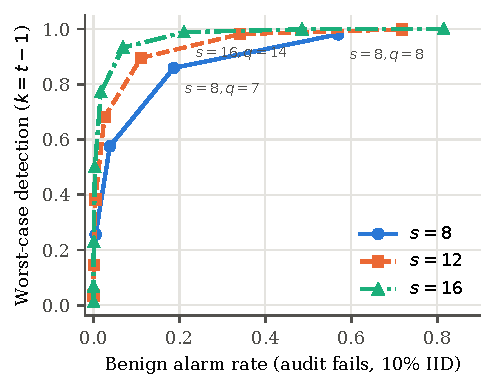
\includegraphics[width=0.62\textwidth]{fig6_acceptance_tradeoff.pdf}
\caption{Detection versus benign alarm rate (the audit fails while the committee is healthy, $f=0.10$) for each $q$, one curve per sample size. Exact values from Table~1 of the article and its full source grid.}
\label{fig:s-acceptance}
\end{figure}

\begin{table}[ht]
\caption{Scalability (R1 prototype, ffdhe groups) with $t=n-\lfloor(n-1)/3\rfloor$. Detection is exact (Eq.~(2) of the article, $q=s$). Audit CPU is $s$ proofs plus $s$ verifications; bytes are one request plus $s$ responses. Dispute time is measured verification of $t$ partials plus combination.}
\label{tab:s-scal}
\centering
\small
\begin{tabular}{@{}rrrrrrrr@{}}
\toprule
 & & & & \multicolumn{2}{c}{Audit, ffdhe2048} & \multicolumn{2}{c}{Dispute: verify $t$ + combine}\\
\cmidrule(lr){5-6}\cmidrule(lr){7-8}
$n$ & $t$ & $s$ & Detection & CPU & Bytes & ffdhe2048 & ffdhe3072\\
\midrule
16 & 11 & 4 & 88.46\% & 1063\,ms & 4,819 & 1585\,ms & 5040\,ms\\
32 & 22 & 8 & 98.07\% & 2125\,ms & 9,415 & 3213\,ms & 10201\,ms\\
64 & 43 & 12 & 99.66\% & 3188\,ms & 14,011 & 6230\,ms & 20086\,ms\\
128 & 86 & 16 & 99.92\% & 4250\,ms & 18,607 & 12534\,ms & 40201\,ms\\
\bottomrule
\end{tabular}

\end{table}

\begin{table}[ht]
\caption{Bulletin-board gas per operation, measured with Foundry 1.5.1 and Solidity 0.8.24 (test-body gas; fixture setup excluded), in the small harness committee named in the scope column; values are deterministic.}
\label{tab:s-gas}
\centering
\footnotesize
\begin{tabularx}{\textwidth}{@{}l r X@{}}
\toprule
Bulletin-board operation & Gas & Harness scope\\
\midrule
Register epoch & 223,629 & n=5, t=3; duplicate-identity validation enabled\\
Open audit & 125,107 & three sampled members; q=3\\
Submit audit response & 57,882 & first commitment from one sampled custodian\\
Mark invalid response & 27,704 & admin records a non-zero evidence hash\\
Record equivocation & 51,710 & second conflicting commitment from one custodian\\
Finalize audit & 29,142 & two responses for a three-member sample after deadline\\
Open dispute & 144,149 & n=5, t=3; all members eligible\\
Cancel request & 5,709 & admin cancels one open audit\\
\bottomrule
\end{tabularx}

\end{table}

\begin{table}[ht]
\caption{Mechanisms that check some form of availability or readiness. ``Secret-key operation'' means the check makes a custodian apply its secret share. Entries describe the mechanism class, not every system in it.}
\label{tab:s-related}
\centering
\footnotesize
\begin{tabularx}{\textwidth}{@{}>{\raggedright\arraybackslash}p{0.27\textwidth}>{\raggedright\arraybackslash}X>{\raggedright\arraybackslash}p{0.17\textwidth}>{\raggedright\arraybackslash}p{0.17\textwidth}@{}}
\toprule
Mechanism & What is checked & Secret-key operation & Deadline evidence\\
\midrule
Liveness heartbeat & A process answers & No & No\\
Threshold-wallet heartbeat (tBTC v2)\cite{tbtc2026heartbeat} & The full signing group signs a heartbeat message & Yes (signing) & A failed heartbeat triggers fund migration\\
Proof of custody\cite{feist2021custody} & A validator holds the data it attests to & Secret-dependent bit & Challenge and penalty\\
PoR and PDP\cite{juels2007por,ateniese2007pdp,bowers2009hail} & A server still stores a file & No & No\\
Data-availability sampling\cite{albassam2021fraud,hallandersen2025das} & Published data are retrievable & No & No\\
VSS, PVSS and DKG transcripts\cite{feldman1987vss,schoenmakers1999pvss,gennaro2007dkg} & Shares were distributed consistently & At setup only & No\\
Threshold-release systems\cite{kokoriskogias2020calypso,stengele2021ethtid,bebel2022ferveo} & A release is performed when requested & At release only & System-specific\\
KEYSTONE & $q$ of $s$ sampled custodians can apply their shares now; $t$ custodians serve a dispute by $\Delta_d$ & Before release (canary) and at release & Bulletin board\\
\bottomrule
\end{tabularx}
\end{table}

\begin{table}[ht]
\caption{Readiness checks compared (R1 prototype). Costs are R1 medians for ffdhe2048; bytes are canonical request plus response transcripts.}
\label{tab:s-baselines}
\centering
\footnotesize
% The table cites the article's Eq. (2); render that reference as the article number.
{\renewcommand{\ref}[1]{2}\begin{tabularx}{\textwidth}{@{}>{\raggedright\arraybackslash}p{0.17\textwidth}>{\raggedright\arraybackslash}p{0.15\textwidth}>{\raggedright\arraybackslash}p{0.14\textwidth}>{\raggedright\arraybackslash}p{0.17\textwidth}X@{}}
\toprule
Readiness check & Exercises the secret share? & Touches production ciphertext? & Detects a static state with $k=t-1$ ready shares & Cost per check ($n=32$, ffdhe2048, measured)\\
\midrule
Liveness heartbeat & No & No & No: a node that lost its share still answers & 1 message per node; no group operations\\
Share registration (Feldman/PVSS check) & Once, at setup & No & No: says nothing about later share loss & One-time $O(nt)$ exponentiations at epoch setup\\
Full-committee canary probe & Yes & No (canary) & Yes, with probability 1 & 32 proofs + 32 verifications; 8501\,ms CPU; 36,991\,B\\
KEYSTONE sampled canary ($s=q=8$) & Yes, for the sampled members & No (canary) & Yes, with probability 0.9807 (Eq.~\ref{eq:bound}) & 8 proofs + 8 verifications; 2125\,ms CPU; 9,415\,B\\
Decrypt a real record as a test & Yes & Yes: exposes a production record & Yes & $t$ verifications plus a real disclosure; excluded by design\\
\bottomrule
\end{tabularx}
}
\end{table}

\bibliographystyle{unsrtnat}
\bibliography{../references}

\end{document}
